% id: 106-38
% book: 100발100중 3-2 기말 · 01 3-2 기말(원의 성질·통계·부록)
% section: 족집게 마무리 객관식 80선 · Ⅶ-1 대푯값과 산포도
% figure: crop:fig-106-38.png
% answer: ⑤
% answer_source: 답지(빠른정답)
% variant_level: 0 (원본 전사)
% 이 파일은 build.mjs 가 items.json 에서 만든다. 고칠 때는 items.json 을 고친다.
\smash{\raisebox{1.5mm}{\dmkichul{100발100중 3-2 기말 106쪽 38번}}}
\noindent\begin{minipage}[t]{0.58\linewidth}\vspace{0pt}\raggedright 다음은 은지네 반 학생 $25$명이 좋아하는 영화 장르를 조사하여 나타낸 표이다. 이때 이 자료의 최빈값은?\end{minipage}\hfill\begin{minipage}[t]{0.4\linewidth}\vspace{0pt}\centering 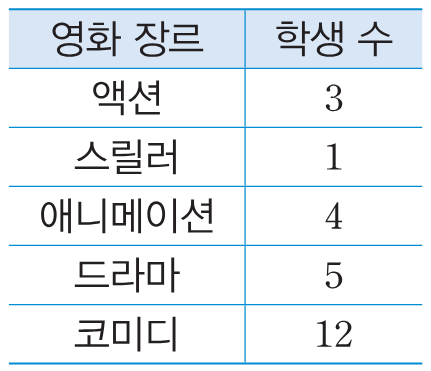
\includegraphics[width=103.2pt]{figures/fig-106-38.png}\end{minipage}\par
\begin{choicesii}{액션}{스릴러}{애니메이션}{드라마}{코미디}\end{choicesii}
